{\color{red}\noindent Red de Datos X.25\\Explicar la arquitectura de X.25}\\

El concepto general del X.25 era crear una red de conmutación de paquetes universal y global. Gran parte del sistema X.25 es una descripción de la rigurosa corrección de errores necesaria para lograr esto, así como un intercambio más eficiente de recursos físicos intensivos en capital. Las redes que utilizan X.25 fueron populares a finales de los años setenta y ochenta entre las empresas de telecomunicaciones y en los sistemas de transacciones financieras, como los cajeros automáticos.

\begin{figure}[ht!]
\centering
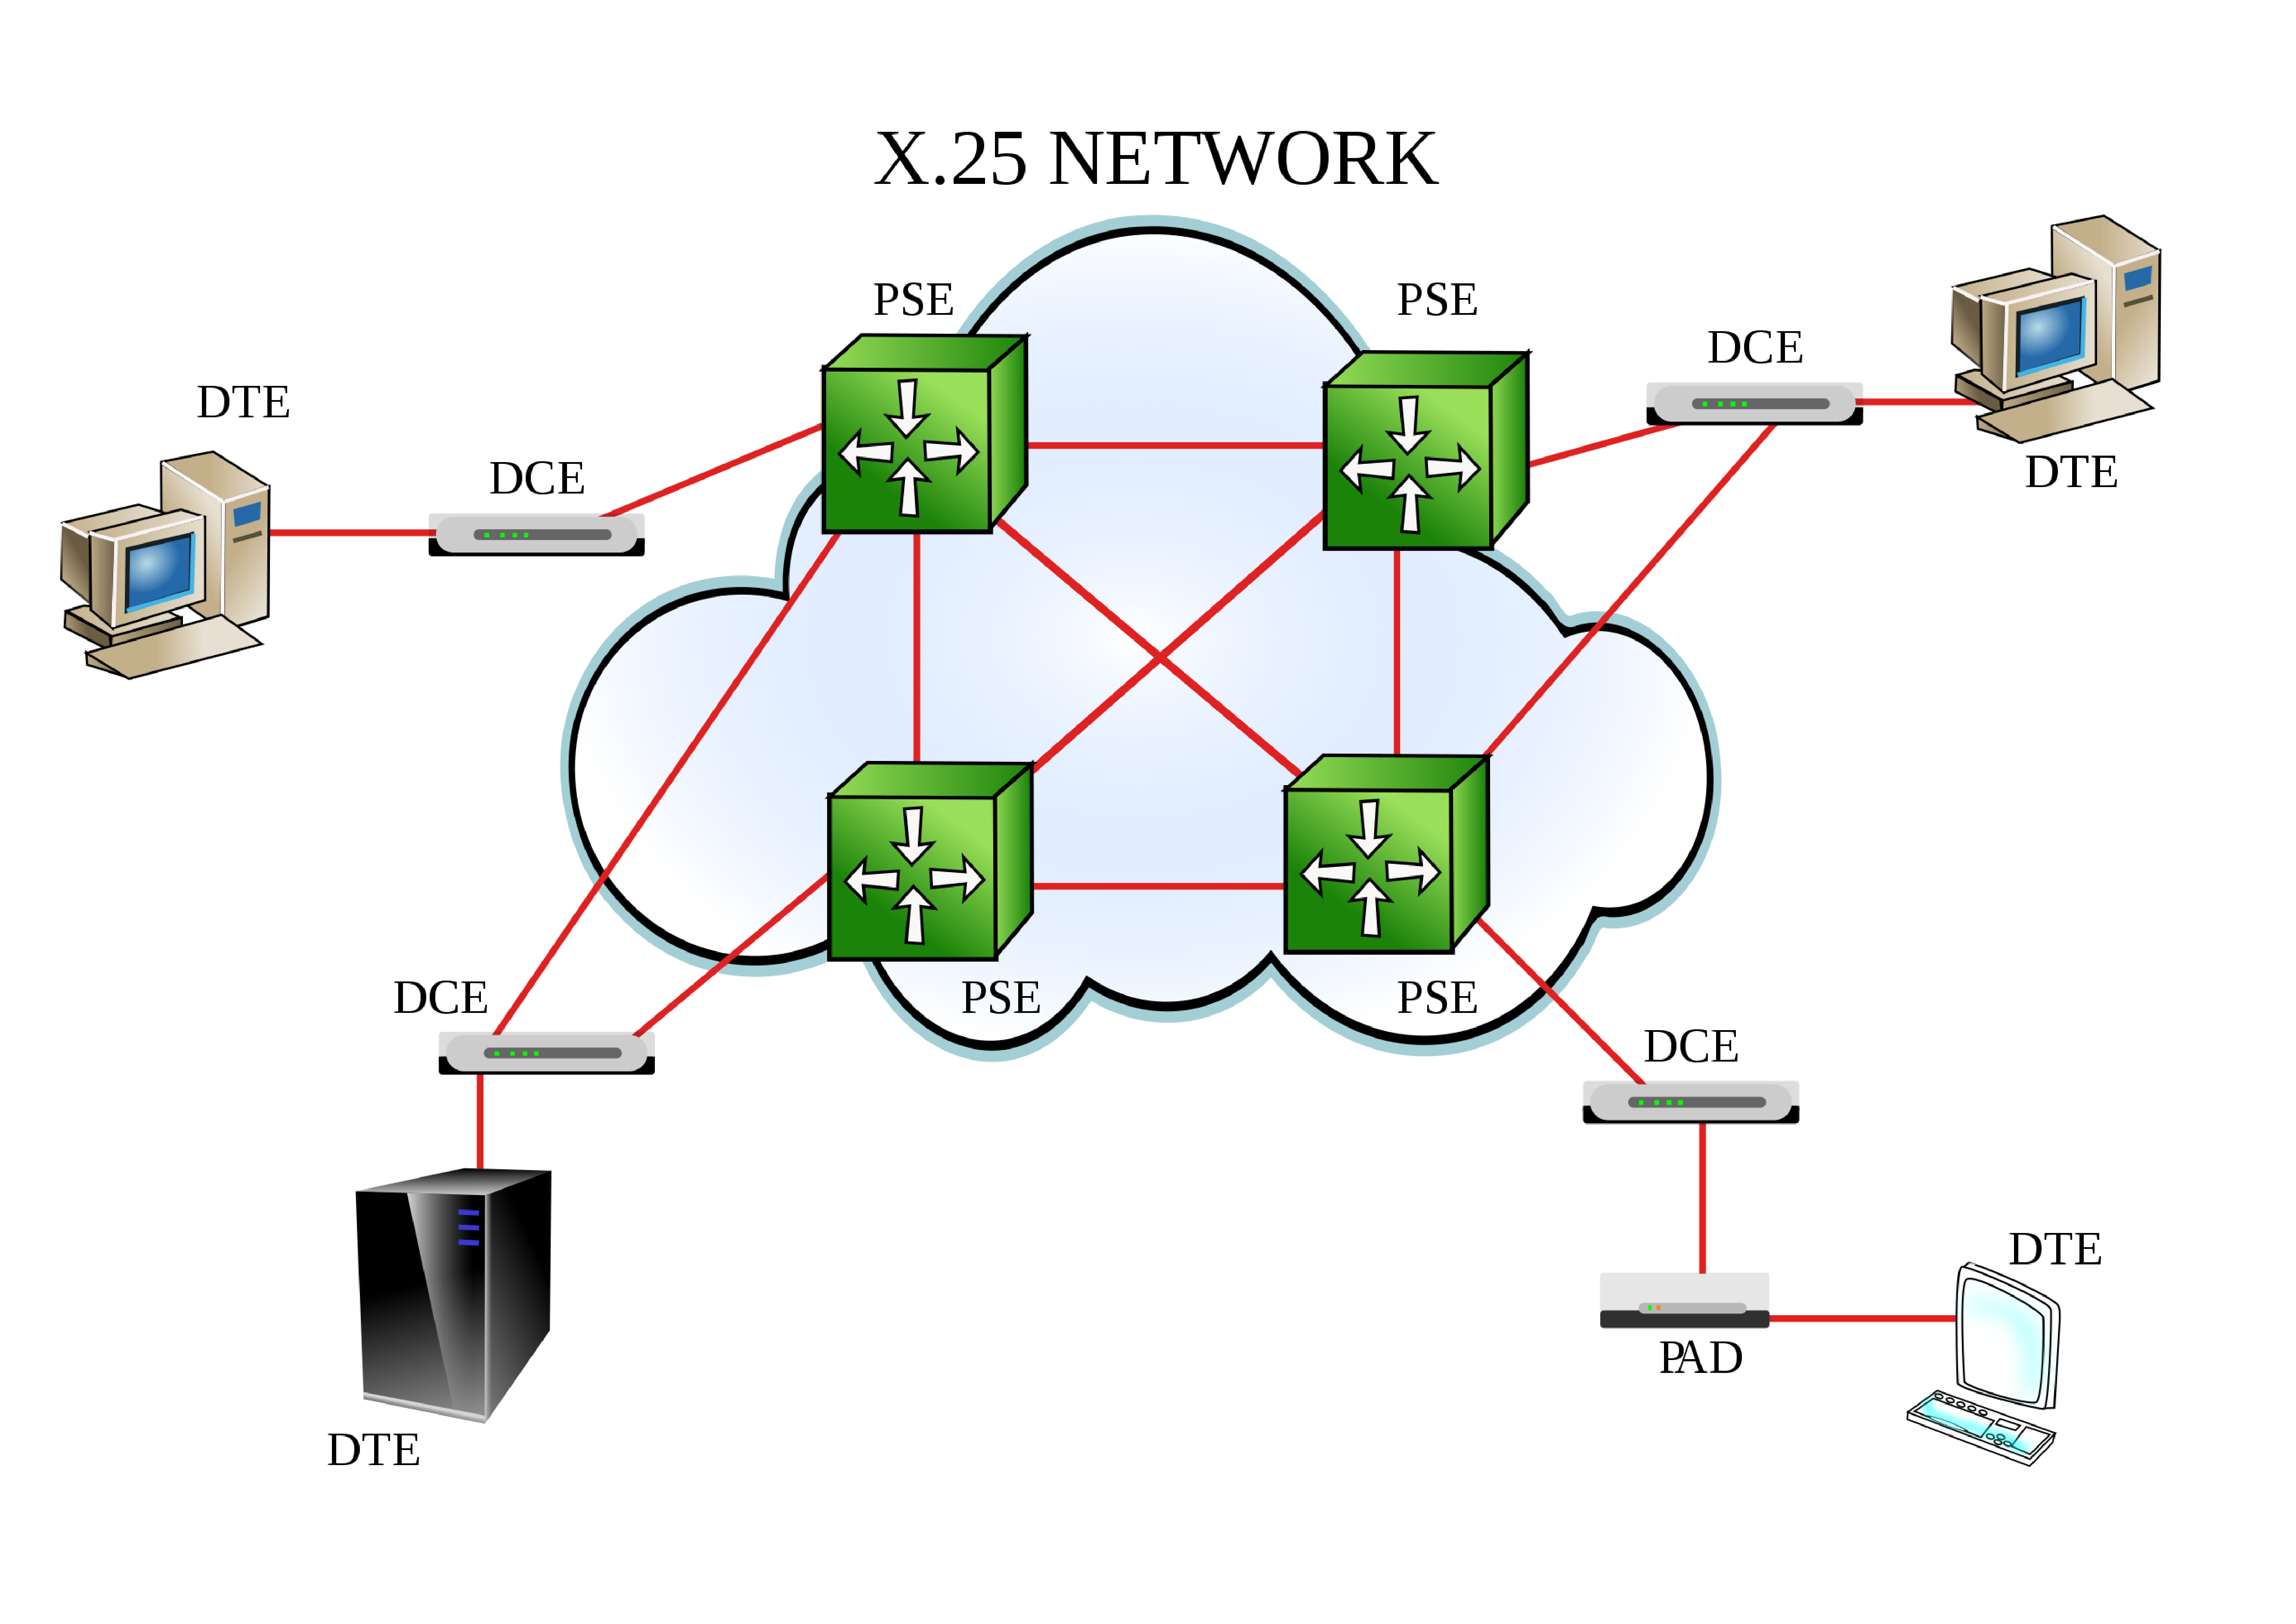
\includegraphics[scale=0.13]{Imagenes/x25.pdf}
\caption{Ejemplo de Arquitectura de X.25}
\end{figure}

Es una interfaz entre \texttt{DTE} y \texttt{DCE} para operar en una red pública de datos en modo paquete. \texttt{DTE} son las siglas de \texttt{Data Terminal Equipment} y \texttt{DCE} son las siglas de \texttt{Data Circuit Terminating Equipment}. X25 es un protocolo de extremo a extremo. El usuario generalmente no se dará cuenta de los paquetes que pasan entre estos terminales.

\subsection*{X.25 Comparado con OSI}
Recordemos que el modelo OSI cuenta con 7 capas; para X.25 podemos distinguir tres: Capa de Paquetes, de Trama y de Física.

\begin{itemize}
\item \textbf{Physical Layer:} Establece las características físicas, eléctricas y funcionales que interactúan entre el terminal de la computadora y el enlace al nodo de conmutación de paquetes.
\item \textbf{Frame Layer:} En esta capa, X.25 proporciona control de enlace de datos mediante LAPB, que es un subconjunto del protocolo HDLC. LAPB es un protocolo orientado a bits. La comunicación es punto a punto y en modo balanceado asíncrono. Aquí se definen dos direcciones,\texttt{ 00000001} y \texttt{00000011}. La primera se utiliza para un comando emitido por \texttt{DTE} y en trama de respuesta a este comando. El segundo es utilizado por el \texttt{DCE} y como trama de respuesta a este comando. Hay tres tipos de tramas: trama-I , trama-S y trama-U.

\begin{figure}[ht!]
\centering
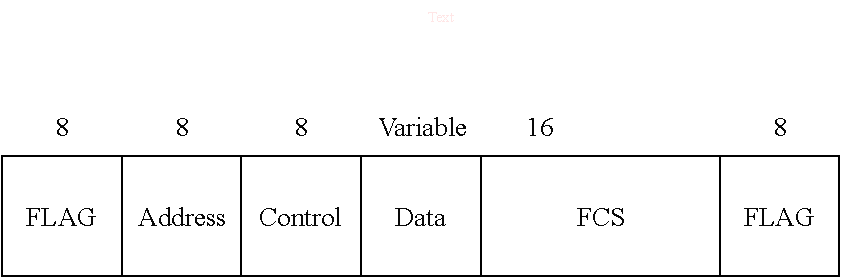
\includegraphics[scale=0.75]{Imagenes/x25lapb.pdf}
\caption{Trama LAPB}
\end{figure}

\subsubsection*{Campo de Control}
El campo Control indica cuál de los tres tipos de tramas LAPB hay:
\begin{itemize}
\item \textbf{Sin numerar (Unnumbered):} establecen y mantienen comunicaciones, hay cinco tipos de tramas-U:
\begin{itemize}
\item \textbf{Set Asynchronous Balanced Mode (Extended) (SABM or SABME)},que establece el enlace DTE a DCE.
\item \textbf{Unnumbered Acknowledgment (UA)}, que confirma la aceptación de una trama.
\item \textbf{Disconnect (DISC)}, desconecta el enlace.
\item \textbf{Disconnect Mode (DM)}, que indica un estado desconectado.
\item \textbf{Frame Reject (FRMR)}, informa una condición de error.
\end{itemize}

\item \textbf{Supervisión: } Permiten el control del flujo de datos y existen tres tipos de tramas S: \textbf{Receiver Ready (RR), Receiver Not Ready (RNR)} y \textbf{Reject (REJ).}
\item  \textbf{Información: } contienen datos, así como recuentos de Próximo Enviado \textbf{(Next Sent: NS)} y Próximo Recibido \textbf{(Next Received: NR)}. La información de secuenciación de las tramas I se superpone, de modo que se agiliza la operación de reconocimiento y un temporizador T1 define cuánto tiempo espera un dispositivo una respuesta.
\end{itemize}


\subsubsection*{Establecer Conexión}
Hay tres fases para establecer la comunicación entre DTE y DCE como se describe a continuación:

\begin{itemize}
\item \textbf{Configuración del enlace:} Primero, es necesario configurar el enlace entre DTE y DCE antes de que se lleve a cabo la transferencia de paquetes. Tanto el DTE como el DCE pueden establecer el enlace enviando una trama SABM y la parte que responde envía una trama UA para indicar que se ha establecido el enlace.
\item T\textbf{ransferencia de datos:} una vez establecido el enlace, ambas partes pueden enviar y recibir tramas de datos/control utilizando tramas-I y tramas-S.
\item \textbf{Desconexión de enlace:} cuando la capa de red ya no necesita la conexión, cualquiera de las partes puede emitir una trama DICS para solicitar la desconexión, la otra parte reconoce emitiendo una trama UA.
\end{itemize}

\item \textbf{Packet Layer:} La capa de red en X25 se denomina protocolo de capa de paquete o capa PLP. Es responsable de establecer la conexión, transferir los datos y terminar la conexión. También es responsable de crear un circuito virtual y negociar los servicios de red entre dos DTE. Como se mencionó, la capa de trama se encarga de la conexión entre DTE y DCE, mientras que la capa de paquetes se encarga de la conexión entre dos DTE. También es responsable de crear un circuito virtual y negociar los servicios de red entre dos DTE. Como se mencionó, la capa de trama se encarga de la conexión entre DTE y DCE, mientras que la capa de paquetes se encarga de la conexión entre dos DTE.
\end{itemize}

\begin{figure}[ht!]
\centering
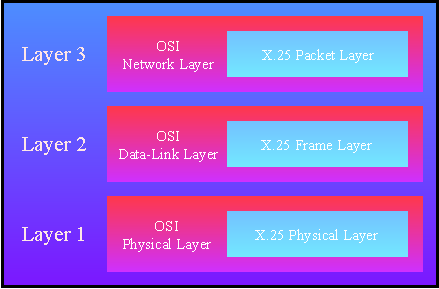
\includegraphics[scale=0.9]{Imagenes/x25layer.pdf}
\caption{OSI vs X.25}
\end{figure}



\begin{thebibliography}{9}

\bibitem{xx}
X.25 - An International Standard. \href{http://clivemabey.me.uk/SciTech/datacomm/x25.php}{http://clivemabey.me.uk/SciTech/datacomm/x25.php}


\bibitem{xx2}
X.25 \href{http://www.rhyshaden.com/x25.htm}{http://www.rhyshaden.com/x25.htm}

\bibitem{xx3}
Link Access Procedure, Balanced (LAPB) Frame Format \href{https://www.geeksforgeeks.org/link-access-procedure-balanced-lapb-frame-format/}{https://www.geeksforgeeks.org/link-access-procedure-balanced-lapb-frame-format/}

\end{thebibliography}

